\section{The Meaning of Necessity}
\label{s:semantics}

 
In this section we define {the}  \Nec specification language.  
We first define an underlying programming language, \Loo (\S \ref{sub:Loo}).
We then define an assertion language, \SpecO, which can talk about the
contents of the state, as well as about provenance, permission and
control (\S \ref{sub:SpecO}).  Finally, we define the syntax and
semantics of our full language for writing \Nec
specifications (\S \ref{s:holistic-guarantees}).


\subsection{\Loo}
\label{sub:Loo} 
%\jm[TODO: mention the type system and the restriction on external method calls]{}
%% We introduce a simple object-oriented language, \Loo, upon 
%% which our specification language sits.
 \Loo is a \jm[removed: formal model of a]{} {small}, imperative, sequential, 
class based, typed, object-oriented language, whose
\sdS{fields are private to the class where they are defined.}
\Loo is straightforward
%Given its simplicity, %  the simplicity of \Loo, we do notdefine it here, instead, 
% we direct the reader to
\jm[]{and the complete definition can be found in the appendices % of the full paper 
\cite{necessityFull}.}
%Appendix \ref{app:loo} contains 
%the full definitions.
%%and introduce here only % syntax and operational semantics.
%% the concepts relevant to the
%%treatment of the open world guarantees.
%\jm[]{\Loo fields are private in the way fields in Java are private,
%the privacy is class-wide, i.e. they may only be read or written to by 
%objects of the same class.}
\Loo is based on \LangOO 
\cite{FASE}, with some small variations, as well as 
the addition of  % while \LangOO is untyped, \Loo 
 a simple type system -- more in \ref{types}.
%has type based restrictions on external access to private data.}
%\sophiaPonder[added]{Note that the operational semantics only allows filed
%update if the receiver and the object being updated belong to the same class,
%and only allows method calls }
%
%
A \Loo state $\sigma$ consists of a 
heap $\chi$, and a  {stack $\psi$ which is a sequence of frames}.
A frame $\phi$ consists of
local variable map, and a continuation, \ie a sequence of statements to be executed.
 A statement may assign to variables, create new objects and push them to the heap, 
perform field reads and writes on objects,  or
 call methods on those objects. 

%Program 
 Modules are mappings
from class names to class definitions. 
Execution 
%takes place
is in the context of  a module $M$ and   a state $\sigma$,
%It is % Execution
 defined via unsurprising small-step semantics of the form \ \ 
   $M, \sigma \leadsto \sigma'$.
The   top frame's continuation contains the statement to be % currently being 
executed next.
 % chopped, as generic 
 % There are several properties  of \Loo that are important to the central topic of this paper. 
 
As discussed in \S \ref{s:approach}, %we are interested in 
{open world specifications need to be able to provide}
guarantees which hold
during execution of an internal, 
known, trusted module $M$ when linked together with any
unknown, untrusted, module $M'$. These guarantees need only hold 
when the external module is executing; we are not concerned if they are
temporarily broken by the internal module. Therefore, we are only interested in states where the
executing object (\prg{this}) is an external object. 
To express our focus on external states, we define the  \emph{external states semantics}, of the form 
$\reduction{M'}{M}{\sigma}{\sigma'}$, where $M'$ is the external
module, and $M$ is the internal module, and where we
collapse all internal steps into one single step.

 

\begin{definition}[External States Semantics]
\label{def:pair-reduce}
For  
% If we say "internal module", it is sounds as something makes the module be internal
  modules $M$,  $M'$, and % program
   states $\sigma$, $\sigma'$, 
we say that $\ \ \ \ \ \ \ \ \reduction{M'}{M}{\sigma}{\sigma'}\ \ \ \ \ \ \ \ $ if and only if there exist 
$n\in\mathbb{N}$, and states $\sigma_0$,...$\sigma_n$, such that
\begin{itemize}
\item
$\sigma$=$\sigma_1$, and  $\sigma'$=$\sigma_n$,
\item
$M' \circ M, \sigma_i \leadsto \sigma_{i+1}$  \ \ \ for all $i\in [0..n)$,
\item
$\class{\sigma}{\scd{\prg{this}}}, \class{\sigma'}{\scd{\prg{this}}}\in M'$,
\item
$\class{\sigma_i}{\scd{\prg{this}}} \in M$\ \ \ for all $i\in (1..n)$.
\end{itemize} 
\end{definition}
The function $\class{\sigma}{\_}$ is overloaded:
  applied to a variable, 
$\class{\sigma}{x}$  looks up the variable $x$ in the top frame of $\sigma$, and returns the 
class of the corresponding object in the  heap of $\sigma$;
%while  
applied to an address, $\class{\sigma}{\alpha}$  returns
the class of   the object referred by address $\alpha$ in the heap of $\sigma$.
 The module linking operator $\circ$, applied to two modules, $M'\circ M$, 
 combines the two modules into one module in the obvious way, provided their
domains are disjoint.
The details \jm[]{can be found in the appendices\cite{necessityFull}.} %Appendix \ref{app:loo}.
\begin{figure}[htb]
\resizebox{0.95\textwidth}{!}{
\begin{tikzpicture}[->,>=stealth',shorten >=1pt,auto,node distance=9mm,
                    thick,
                    external node/.style={circle,draw,minimum size=7mm,font=\sffamily\Large\bfseries, color=blue, fill = blue, text = black, fill opacity = 0.5},
                    internal node/.style={circle,draw,minimum size=7mm,font=\sffamily\Large\bfseries, color=orange, fill = orange, text = black, fill opacity = 0.5}]
    
	\node[external node] (a) {1};
	\node[internal node] (b) [right = of a] {2};
	\node[external node] (c) [right = of b] {3};
	\node[external node] (d) [right = of c] {4};
	\node[internal node] (e) [right = of d] {5};
	\node[internal node] (f) [right = of e] {6};
	\node[external node] (g) [right = of f] {7};
	\node[internal node] (h) [right = of g] {8};
	\node[external node] (i) [right = of h] {9}; 

	\path[every node/.style={font=\sffamily\small}]
		(a) edge[bend left] node [above] {} (b)
		(b) edge[bend left] node [above] {} (c)
		(c) edge[bend left] node [above] {} (d)
		(d) edge[bend left] node [above] {} (e)
		(e) edge[bend left] node [above] {} (f)
		(f) edge[bend left] node [above] {} (g)
		(g) edge[bend left] node [above] {} (h)
		(h) edge[bend left] node [above] {} (i);
\end{tikzpicture}
\begin{tikzpicture}[->,>=stealth',shorten >=1pt,auto,node distance=9mm,
                    thick,
                    external node/.style={circle,draw,minimum size=7mm,font=\sffamily\Large\bfseries, color=blue, fill = blue, text = black, fill opacity = 0.5},
                    internal node/.style={circle,draw,minimum size=7mm,font=\sffamily\Large\bfseries, color=orange, fill = orange, text = black, fill opacity = 0.2, draw opacity = 0.5}]
    
	\node[external node] (a) {1};
	\node[internal node] (b) [right = of a] {2};
	\node[external node] (c) [right = of b] {3};
	\node[external node] (d) [right = of c] {4};
	\node[internal node] (e) [right = of d] {5};
	\node[internal node] (f) [right = of e] {6};
	\node[external node] (g) [right = of f] {7};
	\node[internal node] (h) [right = of g] {8};
	\node[external node] (i) [right = of h] {9}; 

	\path[every node/.style={font=\sffamily\small}]
		(a) edge[bend left=46] node [above] {} (c)
		(c) edge[bend left=46] node [above] {} (d)
		(d) edge[bend left=46] node [above] {} (g)
		(g) edge[bend left=46] node [above] {} (i);
\end{tikzpicture}
}
   \caption{External States Semantics
     (Def. \ref{def:pair-reduce}),  %
     % 
     (A) $\exec{{\color{hotpink}M'} \circ {\color{lightseagreen}M}}{\sigma_1}{\ldots}\leadsto \sigma_9$ \ \ \ and \ \ \ 
     (B) $\reduction{{\color{hotpink}M'}}{{\color{lightseagreen}M}}{\sigma_2}{\ldots}\leadsto \sigma_9$, \ \ \ 
     \\
     where $\class{{\color{lightseagreen}\sigma_1}}{\scd{\prg{this}}}$,$\class{{\color{lightseagreen}\sigma_3}}{\scd{\prg{this}}}$,$\class{{\color{lightseagreen}\sigma_4}}{\scd{\prg{this}}}$,$\class{{\color{lightseagreen}\sigma_7}}{\scd{\prg{this}}}$,$\class{{\color{lightseagreen}\sigma_8}}{\scd{\prg{this}}}\in {\color{lightseagreen}M}$,\\
     and where $\class{{\color{hotpink}\sigma_2}}{\scd{\prg{this}}},\class{{\color{hotpink}\sigma_5}}{\scd{\prg{this}}} 
     \class{{\color{hotpink}\sigma_6}}{\scd{\prg{this}}},\class{{\color{hotpink}\sigma_9}}{\scd{\prg{this}}}\in {\color{hotpink}M'}$.
    %  (c) $\reduction{{\color{orange}M'}}{{\color{blue}M}}{\sigma_1}{\ldots}\leadsto \sigma_8$
    }
   \label{fig:VisibleStates}
 \end{figure}
 
Fig. \ref{fig:VisibleStates} inspired by \citeasnoun{FASE} provides a simple graphical description of 
our external states semantics: (A) is the ``normal'' execution after 
linking two modules into one: \ $M' \circ M, ... \leadsto ...$ whereas (B) is the
 external states execution when $M'$ is external,\   $\reduction{M'}{M}{...}{...}$.
Note that whether a module is external or internal depends on %our
perspective -- nothing in a module itself renders it internal or external. For example, in
 $\reduction{M_1}{M_2}{...}{...}$ the external module is $M_1$,
  while in  $\reduction{M_2}{M_1}{...}{...}$  the external module is $M_2$.

We  use the notation\ \  $\reductions{M'}{M}{\sigma}{\sigma'}$ \ 
to denote zero or more  steps starting at state $\sigma$ and ending at state $\sigma'$, in the context of internal module 
$M$ and external module $M'$.
 %Not only are we unconcerned 
%with internal states,  we are also unconcerned with  states which cannot ever arise from execution.
We are \jm[]{not} concerned with internal states or states that can never arise.
{A state $\sigma$ is \emph{arising},}  written $\arising{M'}{M}{\sigma}$, {if it  may arise by external states} execution
starting at some initial configuration:



\begin{definition}[Arising  States]
\label{def:arising}
For   modules $M$ and  $M'$, a % program
 state $\sigma$ is 
called an \emph{arising} state, formally \ \ \ $\arising{M'}{M}{\sigma}$,\ \ \ 
if and only if there exists some $\sigma_0$ such that $\initial{\sigma_0}$ and
$\reductions{M'}{M}{\sigma_0}{\sigma}$.
\end{definition}

An \emph{Initial} state's heap
contains a single object of class \prg{Object}, and
its  stack   consists of a single frame, whose local variable map is a
mapping from \prg{this} to the single object, and whose continuation is  any statement.
(See Definition %s \ref{def:initial} and 
\ref{def:arising} and the 
\jm[]{appendices %of the full paper 
\cite{necessityFull}).}


\paragraph{Applicability} 
{While our work is based on 
  a simple, imperative, typed, object oriented}
language with unforgeable addresses and private fields, we believe
 that % our approach
 it is applicable to several programming paradigms, and 
 that   unforgeability and privacy
 can be replaced 
 by lower level mechanisms such as capability machines \cite{vanproving,davis2019cheriabi}.

\subsection{\SpecO}
\label{sub:SpecO}

\SpecO is \jm[removed: a subset of the \emph{Chainmail} assertions language, \ie]{}
a basic assertion language extended with
object-capability assertions. 


\subsubsection{Syntax of \SpecO}
The syntax of \SpecO   is given in
Definition \ref{f:chainmail-syntax}.
An assertion may be an expression,   a query of the defining class of
  an object, the usual connectives and quantifiers, along 
with three non-standard assertion forms:
(1) \emph{Permission} and (2) \emph{Provenance}, inspired by the capabilities literature, and
(3) \emph{Control} which allows tighter  characterisation of the cause of effects --  
useful for the specification of large APIs.
\begin{itemize}
\item
\emph{Permission} ($\access{x}{y}$):  
  $x$ has access to $y$.
\item
{\emph{Provenance}} ($\internal{x}$ and $\external{y}$):   $x$ is an internal \jm[]{(i.e. trusted) object}, and $y$ is an external \jm[]{(i.e. untrusted) object}.
\item
\emph{Control} ($\calls{x}{y}{m}{\overline{z}}$): 
$x$ calls method $m$ on object $y$ with arguments $\overline{z}$.
\end{itemize}


\begin{definition}
Assertions ($A$) in
\SpecO are defined as follows:

\label{f:chainmail-syntax}
 \[
\begin{syntax}
\syntaxElement{A}{}
		{
		\syntaxline
				{e}
				{e : C}
				{\neg A}
				{A\ \wedge\ A}
				{A\ \vee\ A}
				{\all{x}{A}}
				{\ex{x}{A}}
		\endsyntaxline
		}
		{
		\syntaxline
				{\access{x}{y}}
				{\internal{x}}
				{\external{x}}
%		\endsyntaxline
%		}
%		{
%		\syntaxline
				{\calls{x}{y}{m}{\overline{z}}}
		\endsyntaxline
		}
\endSyntaxElement\\
\end{syntax}
\]


\end{definition}



\subsubsection{Semantics of \SpecO}
The semantics of \SpecO   
is given in Definition \ref{def:chainmail-semantics}. 
We   use the evaluation relation, $\eval{M}{\sigma}{e}{v}$,
which says that the expression $e$ evaluates
to value $v$ in the context of state $\sigma$ and module $M$.
Note that expressions in \Loo may be recursively defined, and thus evaluation 
need not \jm[removed: always]{} % may not necessarily 
 terminate. Nevertheless, the logic of $A$ remains classical because recursion is restricted
to expressions, and not generally to assertions.
We have taken this approach from \citeasnoun{FASE}, which also contains a mechanized Coq proof that assertions are classical \cite{coqFASE}.
%  The full
The semantics of $\hookrightarrow$ \jm[]{is} unsurprising 
(see \jm[]{the appendices %of the full paper 
\cite{necessityFull}).} %Fig.\ref{f:evaluation}).

Shorthands: 
 $\interpret{\phi}{x} = v$  means that $x$ maps to
value $v$ in the local variable map of frame $\phi$, $\interpret{\sigma}{x} = v$ means that $x$ 
maps to $v$ in the top most frame of $\sigma$'s stack, and $\interpret{\sigma}{x.f} = v$
has the obvious meaning. The terms $\sigma.\prg{stack}$,  
%resp. 
$\sigma.\prg{contn}$, 
%resp. 
$\sigma.\prg{heap}$     mean the stack, 
%resp. 
the continuation at the
top frame of $\sigma$, %resp. 
and the heap of $\sigma$.
The term $\alpha\!\in\!\sigma.\prg{heap}$ means that $\alpha$ is in the domain of the heap of $\sigma$, and \emph{$x$ fresh in $\sigma$} means that 
$x$ isn't in the variable map of the top frame of $\sigma$, 
while the substitution  $\sigma[x \mapsto \alpha]$ is applied to the top frame of $\sigma$.
\jm[added extra space]{\ }$C\in M$ means that class $C$ is in the domain of module $M$. 

\begin{definition}[Satisfaction % of \SpecO 
of Assertions by a module and a state] 
\label{def:chainmail-semantics}
We define satisfaction of an assertion $A$ by a % program 
state $\sigma$ with 
 module $M$ as:
\begin{enumerate}
\item
\label{cExpr}
$\satisfiesA{M}{\sigma}{e}$ \ \ \ iff \ \ \  $\eval{M}{\sigma}{e}{\true}$
\item
\label{cClass}
$\satisfiesA{M}{\sigma}{e : C}$ \ \ \ iff \ \ \  $\eval{M}{\sigma}{e}{\alpha}$ \textit{and} $\class{\sigma}{\alpha} = C$
\item
$\satisfiesA{M}{\sigma}{\neg A}$ \ \ \ iff \ \ \  ${M},{\sigma}\nvDash{A}$
\item
$\satisfiesA{M}{\sigma}{A_1\ \wedge\ A_2}$ \ \ \ iff \ \ \  $\satisfiesA{M}{\sigma}{A_1}$ and 
$\satisfiesA{M}{\sigma}{A_2}$
\item
$\satisfiesA{M}{\sigma}{A_1\ \vee\ A_2}$ \ \ \ iff \ \ \  $\satisfiesA{M}{\sigma}{A_1}$ or 
$\satisfiesA{M}{\sigma}{A_2}$
\item
\label{quant1}
$\satisfiesA{M}{\sigma}{\all{x}{A}}$ \ \ \ iff \ \ \  
$\satisfiesA{M}{\sigma[x \mapsto \alpha]}{A}$, \ 
\ \ \ for some $x$ fresh in $\sigma$, and for all $\alpha\!\in\!\sigma.\prg{heap}$.
\item
\label{quant2}
$\satisfiesA{M}{\sigma}{\ex{x}{A}}$ \ \ \ iff \ \ \  
$\satisfiesA{M}{\sigma[x \mapsto \alpha]}{A}$, \ 
\ \ for some $x$ fresh in $\sigma$, and for some $ \alpha\!\in\!\sigma.\prg{heap}$. 
\item
\label{cAccess}
$\satisfiesA{M}{\sigma}{\access{x}{y}}$ \ \ \ iff \ \ \  
\begin{enumerate}
\item
\label{c1}
$\interpret{\sigma}{x.f}={\interpret{\sigma}{y}}$ for some $f$, \\
  or
\item
\label{c2}
{$\interpret{\sigma}{x}=\interpret{\phi}{\prg{this}}$}, {$\interpret{\sigma}{y}=\interpret{\phi}{z}$}, and $z\ \in\ \phi.\prg{contn}$\ \ \ \
for some variable $z$, and some frame $\phi$ in $\sigma.
\prg{stack}$.
\end{enumerate}
\item
\label{cInternal}
$\satisfiesA{M}{\sigma}{\internal{x}}$ \ \ \ iff \ \ \  
$\textit{classOf}(\sigma,x) \in M$
\item
\label{cExternal}
$\satisfiesA{M}{\sigma}{\external{x}}$ \ \ \ iff \ \ \  
$\textit{classOf}(\sigma,x) \not\in M$
\item
\label{cCall}
$\satisfiesA{M}{\sigma}{\calls{x}{y}{m}{z_1, \ldots, z_n}}$ \ \ \ iff \ \ \ 
\begin{enumerate}
\item
$\sigma.\prg{contn} = (w := y'.m(z'_1,\ldots,z'_n)\scd{; s})$,\ \ for some 
variable $w$, and some statement $s$,
\item
$\satisfiesA{M}{\sigma}{x = \prg{this}}$
\ \ and \ \ 
$\satisfiesA{M}{\sigma}{y = y'}$,
\item
$\satisfiesA{M}{\sigma}{z_i = z'_i}$\ \ \ for all $1\!\leq i\!\leq n$
\end{enumerate}
\end{enumerate}
\end{definition}

\julian{Quantification (defined in \ref{quant1} and \ref{quant2}) is done over all objects on the heap.
We do not include quantification over primitive types such as integers as \Loo is too simple. The 
Coq mechanisation does include primitive types.}
 
The assertion ${\access{x}{y}}$ (defined in  \ref{cAccess})
requires  that $x$ has access to $y$
either through a field of $x$ (case \ref{c1}),
or through some call in the stack, where $x$ is the receiver and $y$ is one of the
arguments (case \ref{c2}).
{Note that access is not deep, and only refers to objects that 
an object has direct access to via a field or within the context of a current scope. 
%A transitive definition of access would not be useful in specifying safe and robust software.
 The restricted form of access used in \Nec specifically captures a crucial property of robust programs in the open world: access to an object does not imply access to that object's internal data. For example, an object may have access to an account \prg{a}, but a safe implementation of the account would never allow that object to leverage that access to gain direct access to {\prg{a.pwd}}}.
 %Necessity is thus concerned with if and how objects are able to gain direct access to an object, and not deep, transitive access. Indeed, if access were defined transitively, then many objects would be defined as having access to objects that they could not gain a direct reference to, and as such render <x access y> as almost meaningless, and any safety specifications written using access to be prohibitively restrictive.
 
 The assertion  %$\satisfiesA{M}{\sigma}
 ${\calls{x}{y}{m}{z_1, \ldots, z_n}}$  (defined in \ref{cCall})
\sdM{describes the current innermost active call}. It
requires that the current receiver (\prg{this}) is $x$, and that it calls the method $m$ on $y$ with
 arguments $z_1$, ... $z_n$ -- It does \emph{not} mean  that somewhere in the 
 call stack there exists a call from $x$ to $y.m(...)$. 
 Note that in most cases, satisfaction of an assertion not only depends on the state $\sigma$, but 
also depends on the module in the case of expressions (\ref{cExpr}), class membership
(\ref{cClass}), and internal or external provenance (\ref{cInternal} and \ref{cExternal}).


We now define what it means for a module to satisfy an assertion:
 $M$ satisfies  $A$ if any state arising from external steps execution of that
module with any other external module  satisfies $A$. 
 
\begin{definition} [Satisfaction % of \SpecO 
of Assertions
by a module] 
\label{def:mdl-sat}
For a module $M$ and assertion $A$, we say that\ \  $\satisfies{M}{A}$ \ \ if and only if 
for all modules $M'$, and all $\sigma$, if $\arising{M'}{M}{\sigma}$, then $\satisfiesA{M}{\sigma}{A}$.
\end{definition}

 
In the current work we assume the existence of a proof system that judges
$\proves{M}{A}$, to prove  satisfaction of assertions. 
 We will not define such a judgement, but will rely on its existence {later on for} Theorem \ref{thm:soundness}.
We define soundness of such a judgement in the usual way:

\begin{definition}[Soundness of \SpecO Provability]
\label{ax:specW-prove-soundness}
A judgement of the form {$\proves{M}{A}$} is \emph{sound}, if for all
 modules $M$ and assertions $A$, \ if $\proves{M}{A}$ then $\satisfies{M}{A}$.
\end{definition}

 
\subsubsection{Inside}

We define
a final shorthand 
predicate $\wrapped{\prg{o}}$ which states 
that only \internalO objects have access to \prg{o}.
The object \prg{o} may be either \internalO or \externalO.
\begin{definition}[Inside]
$\wrapped{o}\ \triangleq\ \all{x}{\access{x}{o}\ \Rightarrow\ \internal{x}} $ 
\end{definition}

 
\inside is a very useful concept. For example, the balance of an account whose
  password is \inside  will not decrease in the next step.
  Often, API implementations contain objects whose capabilities, while  crucial for the implementation, if exposed,
would break the intended guarantees of the API. Such objects need to remain \inside - see
such an example in Section \ref{s:examples}. 
 


\subsection {\Nec operators}
\label{s:holistic-guarantees}

\subsubsection{Syntax of \Nec Specifications}
The \Nec specification language extends \SpecO with our three novel 
 \jm[]{\Nec} \emph{operators}:

\begin{description}
\item %[Single-Step Only If]
[$\onlyIfSingle{A_1}{A_2}{A}$]: If an arising  
  state satisfies $A_1$, and \sd{a single execution step reaches}  a state satisfying $A_2$, 
then the original  
state must have also satisfied $A$.

\item %[Only If]
[$\onlyIf{A_1}{A_2}{A}$]: If an arising  
  state satisfies $A_1$ and \sd{a number of execution steps reach} a state   satisfying $A_2$, 
then the original  
state must have also satisfied $A$.

\item %[Only Through]
[$\onlyThrough{A_1}{A_2}{A}$]: If an arising  
 state satisfies $A_1$, and \sd{a number of execution steps reach} a state  
 satisfying $A_2$,  then  execution must have passed through some \emph{intermediate} state satisfying $A$.
\end{description}


\noindent
The syntax of  \Nec specifications is given below

\begin{definition}  

\noindent
{\emph{\sd{Syntax of \Nec Specifications}}}

\label{f:holistic-syntax}
\footnotesize
\[
\begin{syntax}
\syntaxElement{S}{}
		{
		\syntaxline
				{A}
				{\onlyIf{A_1}{A_2}{A_3}}
				{\onlyThrough{A_1}{A_2}{A_3}}
		% \endsyntaxline
		% }
		%{
		% \syntaxline
				 {\onlyIfSingle{A_1}{A_2}{A_3}}
		\endsyntaxline
		}
\endSyntaxElement\\
\end{syntax}
\]
%\end{definition}
%%\end{figure}
\normalsize
\end{definition}

\label{sec:adapt:motivate}



\noindent
As an example, we consider the following three  specifications:

\begin{lstlisting}[language = Chainmail, mathescape=true, frame=lines]
$\text{\SRobustNextAcc}$   $\triangleq$  from a:Account $\wedge$ a.balance==bal  next a.balance < bal
                        onlyIf $\exists$ o.[$\external{\texttt{o}}$ $\wedge$ $\access{\prg{o}}{\prg{a.pwd}}$]
$\text{\SRobustIfAcc}$   $\triangleq$  from a:Account $\wedge$ a.balance==bal  to a.balance < bal
                        onlyIf $\exists$ o.[$\external{\texttt{o}}$ $\wedge$ $\access{\prg{o}}{\prg{a.pwd}}$]
$\text{\SRobustThroughAcc}$   $\triangleq$  from a:Account $\wedge$ a.balance==bal  next a.balance < bal
                        onlyThrough $\exists$ o.[$\external{\texttt{o}}$ $\wedge$ $\access{\prg{o}}{\prg{a.pwd}}$]                                   
\end{lstlisting}

\noindent
\SRobustNextAcc  requires that an account's balance may decrease in \emph{one step} (go from a state where the balance is \prg{bal}
to a state where it is less than \prg{bal}) only if the password is accessible to an external object (in the original state an external object had access to the password).
\SRobustIfAcc  requires that an account's balance may decrease in \emph{any number of steps}    only if the password is accessible to an external object.
\SRobustThroughAcc requires that an account's balance may decrease in \emph{any number of steps}    only if in \emph{some intermediate state} the password was accessible to an external object --  the   \emph{intermediate} state  where the password is accessible to the external object might be the \emph{starting}  
state, the \emph{final} state, or any state in between.

 


\subsubsection{Semantics of \Nec Specifications}
We now  define what it means for  a module  $M$ to satisfy specification  $S$, written as $M \vDash S$. The
 Definition~\ref{def:necessity-semantics} below is straightforward, apart from  
the use of the $\adapt  {\sigma'}{\sigma}$  (best read as ``$\sigma'$ seen
from $\sigma$'')
% although one recalcitrant author prefers ``$\sigma'$adapted to $\sigma$'') 
% our reviewers did not appreciate the jokes
to deal with the fact that execution might  change the bindings in local variables.
We explain this in detail in   \S \ref{sub:adapt:full}, but for now, the reader may ignore the applications of that operator and
read $\sigma' \triangleleft \sigma$ as $\sigma'$,
and also read ${\sigma_k \triangleleft \sigma_1}$ as  $\sigma_k$.
We illustrate the meaning of the three operators in 
Fig.~\ref{fig:Operators}.

%
%
\begin{figure}[htbp]
\resizebox{0.95\textwidth}{!}{
% \begin{minipage}{0.50\textwidth}
\newcommand{\mathsmall}[1]{\substack{\scalebox{0.8}{$#1$}}}
\begin{minipage}{\textwidth}
$\onlyIf{A_1}{A_2}{A}$:\\\\
\begin{tikzpicture}[->,>=to,shorten >=1pt,auto,node distance=5.5mm,
                    thick,
                    state/.style={circle,draw,minimum size=5mm,font=\sffamily\bfseries, color=hotpink, fill = hotpink, text = black, fill opacity = 0.5, scale=0.9},
                    dots/.style={
                    minimum size=7mm,
                    font=\sffamily\Large\bfseries, 
                    color=lightseagreen, text = black, fill opacity = 0.5},
                    space/.style={
                    minimum size=7mm,
                    font=\sffamily\Large\bfseries, 
                    color=lightseagreen, text = black, fill opacity = 0.5},
                    arrow/.style={
                    minimum size=7mm,
                    font=\sffamily\Large\bfseries, 
                    color=lightseagreen, text = black, fill opacity = 0.5},
                    models/.style={
                    minimum size=7mm,
                    font=\sffamily\Large\bfseries, 
                    color=lightseagreen, text = black, fill opacity = 0.5},
                    decoration = snake]
    
	\node[state, label={270:$\mathsmall{\vDash A_1}$}] (la) {$\sigma_1$};
	\node[space] (s1) [right = of la] {};
	\node[dots] (lb) [right = of s1] {$\ldots$};
	\node[space] (s2) [right = of lb] {};
	\node[state, label={270:$\mathsmall{\vDash A_2}$}] (lc) [right = of s2] {$\sigma_n$};
	\draw [decorate, ->]
	(la) -- (s1);
	\draw [decorate, ->]
	(s2) -- (lc);

	\node[arrow] (c) [right = of lc] {$\Longrightarrow$};
    
	\node[state, label={270:$\mathsmall{\vDash A_1 \color{hotpink}{\mathbf{\wedge A}}}$}] (ra) [right = of c] {$\sigma_1$};
	\node[space] (s3) [right = of ra] {};
	\node[dots] (rb) [right = of s3] {$\ldots$};
	\node[space] (s4) [right = of rb] {};
	\node[state, label={270:$\mathsmall{\vDash A_2}$}] (rc) [right = of s4] {$\sigma_n$};

	\draw [decorate, ->]
	(ra) -- (s3);
	\draw [decorate, ->]
	(s4) -- (rc);
\end{tikzpicture}\\\\
$\onlyIfSingle{A_1}{A_2}{A}$:\\\\
\begin{tikzpicture}[->,>=to,shorten >=1pt,auto,node distance=5.5mm,
                    thick,
                    state/.style={circle,draw,minimum size=7mm,font=\sffamily\bfseries, color=hotpink, fill = hotpink, text = black, fill opacity = 0.5, scale=0.9},
                    dots/.style={
                    minimum size=7mm,
                    font=\sffamily\Large\bfseries, 
                    color=lightseagreen, 
                    text = black, 
                    fill opacity = 0.5},
                    space/.style={
                    minimum size=7mm,
                    font=\sffamily\Large\bfseries, 
                    color=lightseagreen, 
                    text = black, 
                    fill opacity = 0.5},
                    arrow/.style={
                    minimum size=7mm,
                    font=\sffamily\Large\bfseries, 
                    color=lightseagreen, 
                    text = black, 
                    fill opacity = 0.5},
                    models/.style={
                    minimum size=7mm,
                    font=\sffamily\Large\bfseries, 
                    color=lightseagreen, 
                    text = black, 
                    fill opacity = 0.5},
                    decoration = snake]
    
    \node[space] (s) at (0,0) {};
	\node[state, label={270:$\mathsmall{\vDash A_1}$}] (a) at (3.85,0) {$\sigma_1$};
%	\node[space] (b) [right = of a] {};
	\node[state, label={270:{$\mathsmall{\vDash A_2}$}}] (c) [right = of a] {$\sigma_n$};
	\draw [decorate, ->]
	(a) -- (c);

	\node[arrow] (d) [right = of c] {$\Longrightarrow$};
    
	\node[state, label={270:$\mathsmall{\vDash A_1 \color{hotpink}{\mathbf{\wedge A}}}$}] (e) [right = of d] {$\sigma_1$};
%	\node[space] (f) [right = of e] { };
	\node[state, label={270:$\mathsmall{\vDash A_2}$}] (g) [right = of e] {$\sigma_n$};

	\draw [decorate, ->]
	(e) -- (g);
\end{tikzpicture}\\\\
$\onlyThrough{A_1}{A_2}{A}$:\\\\
\begin{tikzpicture}[->,>=to,shorten >=1pt,auto,node distance=5.5mm,
                    thick,
                    state/.style={circle,draw,minimum size=7mm,font=\sffamily\bfseries, color=hotpink, fill = hotpink, text = black, fill opacity = 0.5, scale=0.9},
                    dots/.style={
                    minimum size=7mm,
                    font=\sffamily\Large\bfseries, color=lightseagreen, text = black, fill opacity = 0.5},
                    space/.style={
                    minimum size=7mm,
                    font=\sffamily\Large\bfseries, color=lightseagreen, text = black, fill opacity = 0.5},
                    arrow/.style={
                    minimum size=7mm,
                    font=\sffamily\Large\bfseries, color=lightseagreen, text = black, fill opacity = 0.5},
                    models/.style={
                    minimum size=7mm,
                    font=\sffamily\Large\bfseries, color=lightseagreen, text = black, fill opacity = 0.5},
                    decoration = snake]
    
	\node[state, label={270:$\mathsmall{\vDash A_1}$}] (la) {$\sigma_1$};
	\node[space] (s1) [right = of la] {};
	\node[dots] (lb) [right = of s1] {$\ldots$};
	\node[space] (s2) [right = of lb] {};
	\node[state, label={270:$\mathsmall{\vDash A_2}$}] (lc) [right = of s2] {$\sigma_n$};
	\draw [decorate, ->]
	(la) -- (s1);
	\draw [decorate, ->]
	(s2) -- (lc);

	\node[arrow] (c) [right = of lc] {$\Longrightarrow$};
    
	\node[state, label={270:$\mathsmall{\vDash A_1}$}] (ra) [right = of c] {$\sigma_1$};
	\node[dots] (d1) [right = of ra] {$\ldots$};
	\node[state, label={270:$\mathsmall{\mathbf{\color{hotpink}{\vDash A}}}$}] (rb) [right = of d1] {$\sigma_k$};
	\node[dots] (d2) [right = of rb] {$\ldots$};
	\node[state, label={270:$\mathsmall{\vDash A_2}$}] (rc) [right = of d2] {$\sigma_n$};

	\draw [decorate, ->]
	(ra) -- (d1);
	\draw [decorate, ->]
	(d1) -- (rb);
	\draw [decorate, ->]
	(rb) -- (d2);
	\draw [decorate, ->]
	(d2) -- (rc);
\end{tikzpicture}
\end{minipage}
%   \end{minipage}
}
\caption{Illustrating the three \Nec operators}
\label{fig:Operators}
\end{figure}





\begin{definition}[Semantics of \Nec Specifications]
We define $\satisfies{M}{{S}}$ by cases over the four possible syntactic forms.
For any assertions   $A_1$, $A_2$, and $A$: \\

\label{def:necessity-semantics}

$\bullet$ \ $\satisfies{M}{{A}}$ \ \ \ iff\ \ \ for all $M'$, $\sigma$,\ if $\arising{M'}{M}{\sigma}$, then $\satisfiesA{M}{\sigma}{A}$. (see Def. \ref{def:mdl-sat})\\

%$\bullet$ \ $\satisfies{M}{{A}}$ \ \ \ as defined in \ref{def:mdl-sat} \\

$\bullet$ \ $\satisfies{M}{\onlyIf {A_1}{A_2}{A}}$ \ \ iff\ \  for all $M'$, $\sigma$, $\sigma'$, such that $\arising{M'}{M}{\sigma}$: \\  

\begin{tabular}{lr}
$\;\;\;\;$- $\satisfiesA{M}{\sigma}{A_1}$  & \rdelim\}{3}{3mm}[$\;\;\;\Rightarrow\;\;\;$  $\satisfiesA{M}{\sigma}{A}$] \\
$\;\;\;\;$- $\satisfiesA{M}{\sigma' \triangleleft \sigma}{A_2}$   \\
$\;\;\;\;$- $\reductions{M'}{M}{\sigma}{\sigma'}$   \\
\end{tabular}\\ 

$\bullet$ \  $\satisfies{M}{\onlyIfSingle {A_1}{A_2}{A}}$\ \ iff\ \   for all $M'$, $\sigma$,   $\sigma'$, such that $\arising{M'}{M}{\sigma}$: \\

\begin{tabular}{lr}
$\;\;\;\;$- $\satisfiesA{M}{\sigma}{A_1}$  & \rdelim\}{3}{3mm}[$\;\;\;\Rightarrow\;\;\;$  $\satisfiesA{M}{\sigma}{A}$] \\
$\;\;\;\;$- $\satisfiesA{M}{\sigma' \triangleleft \sigma}{A_2}$   \\
$\;\;\;\;$- $\reduction{M'}{M}{\sigma}{\sigma'}$   \\
\end{tabular}\\ 
  
$\bullet$ \  $\satisfies{M}{\onlyThrough {A_1}{A_2}{A}}$ \ \ iff\ \  for all $M'$, $\sigma_1$,  \sd{$\sigma_2$,  ....} $\sigma_n$, such that $\arising{M'}{M}{\sigma_1}$: \\

 %\sdr[new version]{
\begin{tabular}{lr}
$\;\;\;\;$- $\satisfiesA{M}{\sigma_1}{A_1}$  & \rdelim\}{3}{3mm}[$\;\;\;\Rightarrow\;\;\;$  $\exists k. \ 1\leq k \leq n \ \wedge \ \satisfiesA{M}{\sigma_k \triangleleft \sigma_1}{A}$]   \\
%$\exists i\!\in\![1..n]. \  \satisfiesA{M}{\sigma_i \triangleleft \sigma_1}{A}$] \\
$\;\;\;\;$- $\satisfiesA{M}{\sigma_n\triangleleft \sigma\sd{_1}}{A_2}$   \\
$\;\;\;\;$- $\forall i\!\in\![1..n).\ \reduction{M'}{M}{\sigma_i}{\sigma_{i+1}}$   \\
\end{tabular} 
%}


\end{definition} 

Revisiting the examples from the previous subsection, we obtain that all three modules satisfy 
$\SRobustNextAcc$. But $\ModB$ does not satisfy $\SRobustIfAcc$: as  already discussed in \S \ref{s:bank}, 
with \prg{a} of class \prg{Account} implemented as in $\ModB$,
starting in a state where no external object has access to \prg{a}'s password, and executing 
\prg{a.set(42); a.transfer(rogue\_account,42)} leads to a state where the balance has decreased.
All three modules satisfy $\SRobustThroughAcc$: namely, in all cases, the balance can only decrease if 
there was a call to \prg{a.transfer(\_,p)} where $\prg{p}=\prg{a.pwd}$, and since that call can only be made from an external object,
\prg{p} is externally known at the time of that call.


 $\begin{array}{llll}
  \   & \ModA \vDash \SRobustNextAcc  \   & \ModB \vDash \SRobustNextAcc \  
  & \ModC \vDash \SRobustNextAcc \\
  \   & \ModA \vDash \SRobustIfAcc  \   & \ModB \nvDash \SRobustIfAcc \  
  & \ModC \vDash \SRobustIfAcc \\
   \   & \ModA \vDash \SRobustThroughAcc  \   & \ModB \vDash \SRobustThroughAcc \  
  & \ModC \vDash \SRobustThroughAcc \\ 
  \end{array}$


\subsubsection{Adaptation}
\label{sub:adapt:full}
We  now discuss  the adaptation operator.  To see the need, 
consider  specification
\begin{lstlisting}[language = Chainmail, mathescape=true, frame=lines]
$\text{\Sadapt}$   $\triangleq$  from a:Account $\wedge$ a.balance==350  next a.balance == 250
                   onlyIf $\exists$ o.[$\external{\texttt{o}}$ $\wedge$ $\calls{\prg{o}}{\prg{a}}{\prg{transfer}}{\prg{\_, \_, \_}}$]
\end{lstlisting}

\sd{Without adaptation,} the semantics of  \Sadapt would be: If
$..,\sigma  \models \prg{a.balance==350}$, 
and  $.., \sigma  \leadsto^* \sigma'$ and $\sigma' \models \prg{a.balance==250}$,
then %  \Sadapt mandates that 
between $\sigma$ and $\sigma'$ there must be
call to   \prg{a.transfer}. 
But if $\sigma$ happened to have another account \prg{a1} with balance
\prg{350}, and if we reach $\sigma'$ from $\sigma$ by executing \prg{a1.transfer(}$..,..$\prg{); a=a1}, then we would 
reach a $\sigma'$ % SD chop as superfluous where $\sigma'\models \prg{a.balance==250}$
\emph{without} \prg{a.transfer} having been called: indeed, without the
account \prg{a} from $\sigma$  having changed at all.
% reviewrs did not appreciate joke
% (Haskell programmers will probably feel at home here).  
\sd{In fact, with such a semantics,  a module would satisfy $\Sadapt$ only if it did not support decrease of \jm[]{the} balance by $100$, or
\jm[]{if} states where an account's balance is \prg{350} were unreachable!}

This is the remit of the adaptation operator: when we consider the
future state, we must ``see it from'' the perspective of the current
state; the binding for variables such as \prg{a} must be from the
current state, even though we may have assigned to them in the mean
time.  Thus, $\adapt {\sigma'} {\sigma}$ keeps the heap from $\sigma'$,
and renames the variables
in the top stack frame of  $\sigma'$ so that all variables defined in $\sigma$ have the same 
bindings
%?  ($\adapt {\sigma'} {\sigma}$)
as in   $\sigma$; the continuation must be adapted similarly (see
Fig.~\ref{fig:Adaptation}).
%
%
%\begin{figure}[tbp]
%\begin{tabular}{clclc}
% \begin{minipage}{0.27\textwidth}
% $\sigma:$\\
%% ~ \\
% 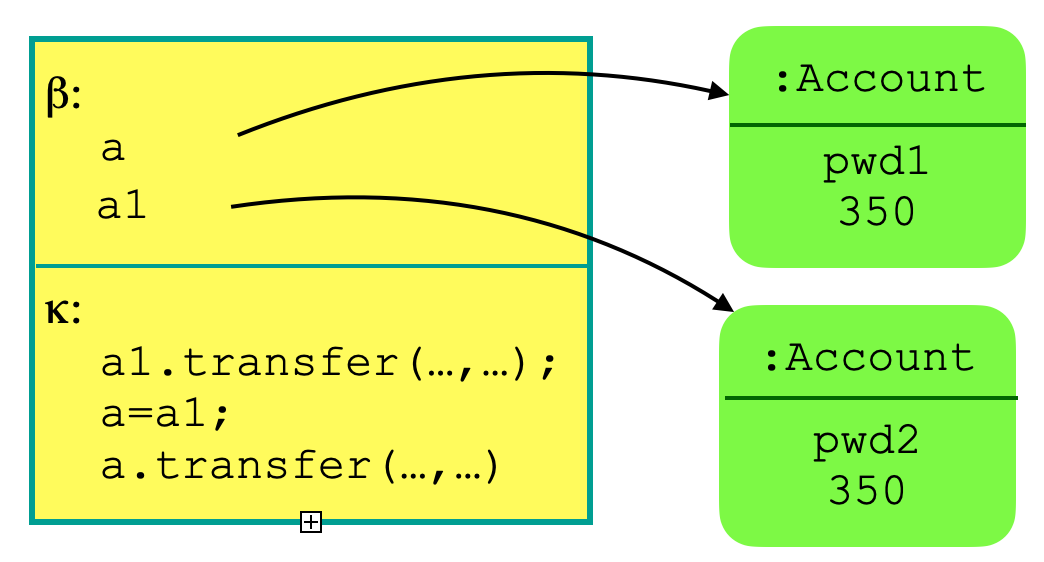
\includegraphics[width=\linewidth]{diagrams/adapt1.png}
%   \end{minipage}
% & \ \ \ &
% \begin{minipage}{0.27\textwidth}
%  $\sigma':$\\
% % ~ \ \\
%  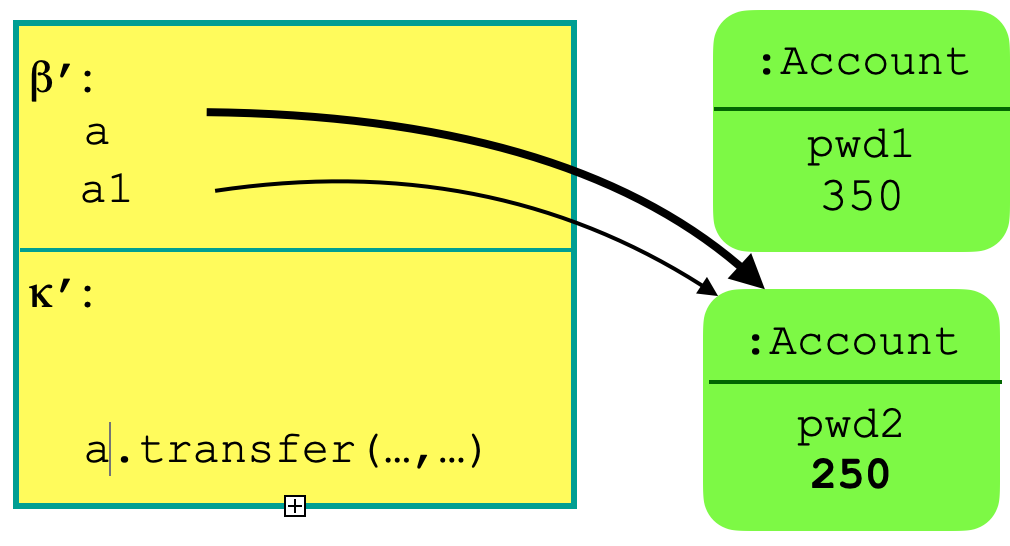
\includegraphics[width=\linewidth]{diagrams/adapt2.png}
%   \end{minipage}
%   & \ \ \  &
%    \begin{minipage}{0.27\textwidth}
%$\adapt {\sigma'}{\sigma}:$\\
%% ~ \\
%  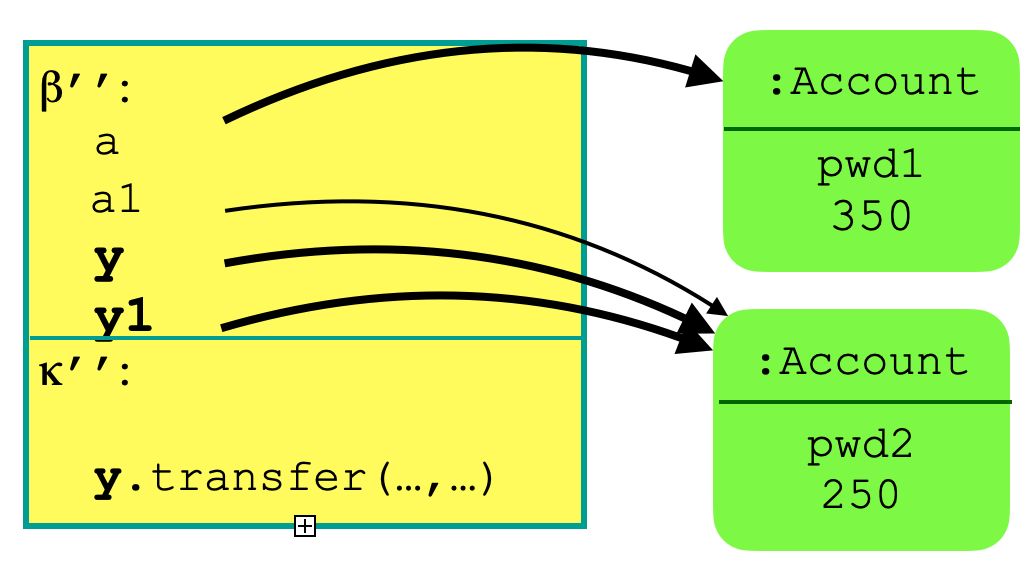
\includegraphics[width=\linewidth]{diagrams/adapt3.png}
%   \end{minipage}
%\end{tabular}
%\caption{Illustrating adaptation
%}
%\label{fig:Adaptation}
%\end{figure}
\newcommand{\mathsmall}[1]{\substack{\scalebox{0.8}{$#1$}}}
\begin{figure}[tbp]
\begin{tabular}{clclc}
 \begin{minipage}{0.27\textwidth}
 $\sigma:$\\
% ~ \\
 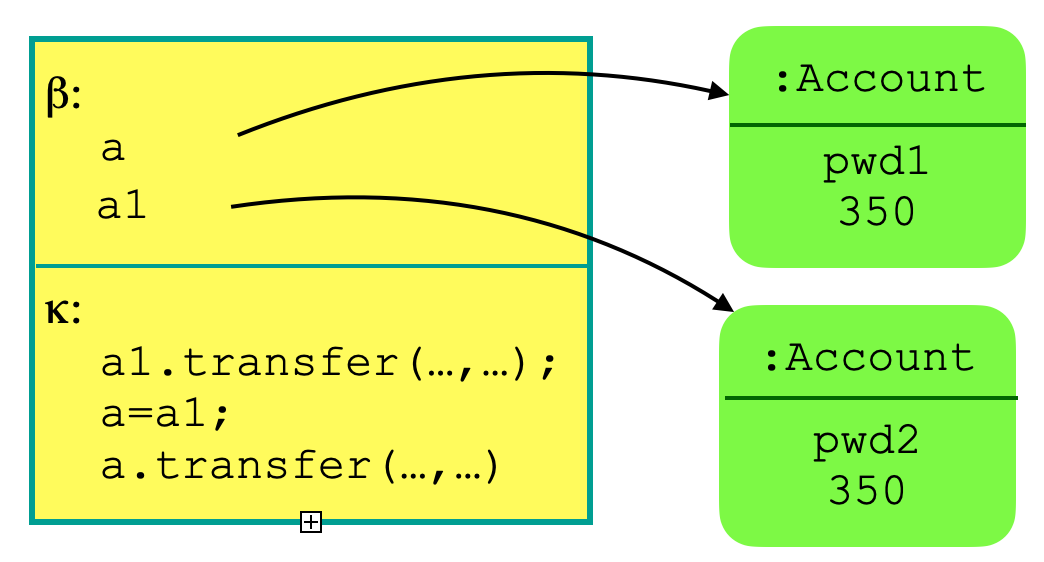
\includegraphics[width=\linewidth]{diagrams/adapt1.png}
   \end{minipage}
 & \ \ \ &
 \begin{minipage}{0.27\textwidth}
  $\sigma':$\\
 % ~ \ \\
  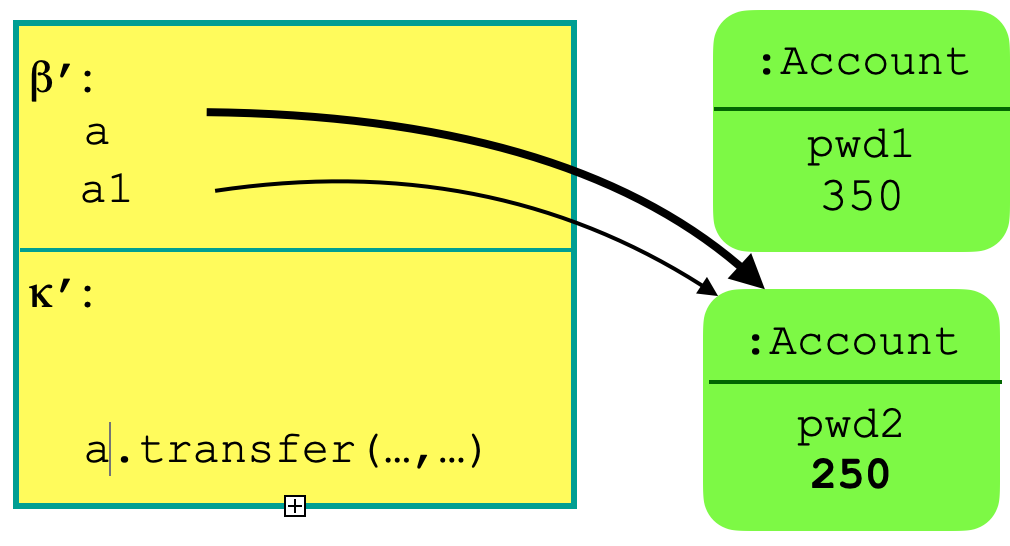
\includegraphics[width=\linewidth]{diagrams/adapt2.png}
   \end{minipage}
   & \ \ \  &
    \begin{minipage}{0.27\textwidth}
$\adapt {\sigma'}{\sigma}:$\\
% ~ \\
  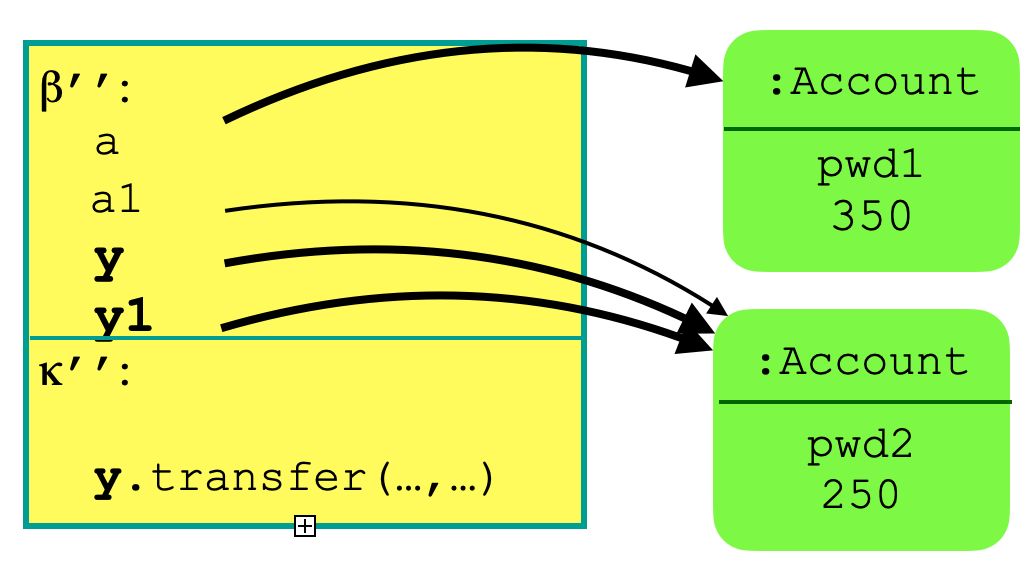
\includegraphics[width=\linewidth]{diagrams/adapt3.png}
   \end{minipage}
\end{tabular}

%\begin{tikzpicture}[->,>=to,shorten >=1pt,auto,node distance=5.5mm,
%                    thick,
%                    state/.style={circle,draw,minimum size=7mm,font=\sffamily\bfseries, color=hotpink, fill = hotpink, text = black, fill opacity = 0.5, scale=0.9},
%                    dots/.style={
%                    minimum size=7mm,
%                    font=\sffamily\Large\bfseries, 
%                    color=lightseagreen, 
%                    text = black, 
%                    fill opacity = 0.5},
%                    space/.style={
%                    minimum size=7mm,
%                    font=\sffamily\Large\bfseries, 
%                    color=lightseagreen, 
%                    text = black, 
%                    fill opacity = 0.5},
%                    arrow/.style={
%                    minimum size=7mm,
%                    font=\sffamily\Large\bfseries, 
%                    color=lightseagreen, 
%                    text = black, 
%                    fill opacity = 0.5},
%                    models/.style={
%                    minimum size=7mm,
%                    font=\sffamily\Large\bfseries, 
%                    color=lightseagreen, 
%                    text = black, 
%                    fill opacity = 0.5},
%                    decoration = snake]
%    
%    \node[space] (s) at (0,0) {};
%	\node[state, label={270:$\mathsmall{\vDash A_1}$}] (a) at (3.85,0) {$\sigma_1$};
%%	\node[space] (b) [right = of a] {};
%	\node[state, label={270:{$\mathsmall{\vDash A_2}$}}] (c) [right = of a] {$\sigma_n$};
%	\draw [decorate, ->]
%	(a) -- (c);
%\end{tikzpicture}
\caption{Illustrating adaptation
}
\label{fig:Adaptation}
\end{figure}




Under adaptation, the semantics of \Sadapt is:\  if $..,\sigma \models \prg{a.balance==350}$,
and  $.., \sigma \leadsto^* \sigma'$ and $..., \boldsymbol{\adapt {\sigma'}{\sigma}} \models \prg{a.balance==250}$,
%then $\sigma_1$'s continuation starts with a call to 
then {some intermediate state's continuation must contain  a call to \prg{a.transfer}};
\sd{where,  all \sd{variables bound in the initial state, $\sigma$,}
have the same bindings in $\adapt {\sigma'}{\sigma}$.}
\jm[I didn't understand susan's comment on this paragraph: ``problem with primes'']{}
 
Fig.~\ref{fig:Adaptation} illustrates the semantics of $\adapt {\sigma'}{\sigma}$. In   $\sigma$ the variable \prg{a} points to an \prg{Account}
 with password \prg{pwd1}, and balance \prg{350};  the variable \prg{a1} points to an \prg{Account}
  with password \prg{pwd2}, and balance \prg{350}; and the continuation is \prg{a1.transfer(}$..,..$\prg{);} \prg{a=a1;}
\prg{a.transfer(}$..,..$\prg{);}. 
We reach $\sigma'$ by executing the first two statements from the continuation.
Thus,  ${\adapt {\sigma'}{\sigma}}\not\models \prg{a.balance==250}$.
Moreover, in $\adapt {\sigma'}{\sigma}$ we introduce the fresh variables \prg{y} and \prg{y1}, and replace \prg{a} and
\prg{a1} by \prg{y} and \prg{y1} in the continuation.
This gives that ${\adapt {\sigma'}{\sigma}} \models \calls {\_} {\prg{a1}} {\prg{transfer}} {...}$ and  ${\adapt {\sigma'}{\sigma}}\not\models \calls {\_} {\prg{a}} {\prg{transfer}} {...}$.

 

Definition~\ref{d:adapt} \sd{describes} the $\adapt{}{}$ operator in all detail
(it is equivalent to, but not identical to the definition  given in \cite{FASE}).
We introduce fresh variables  $\overline{y}$ -- as many as in the $\sigma'$ top frame variable map
-- $dom(\beta')=\overline{x}$,  and $|\overline{y}| = |\overline{x}|$.  
We extend $\sigma$'s variable map ($\beta$), so that it also maps $\overline{y}$ 
in the way that  $\sigma'$'s variable map ($\beta'$) maps its local variables -- $\beta'' =  \beta[\overline{y} \mapsto  {\beta'(\overline{x})}]$. We rename $\overline{x}$   in $\sigma'$ continuation
to $\overline{y}$ --  $\kappa''=[\overline{y}/\overline{x}]\kappa'$.

 
 
\begin{definition}
\label{d:adapt}
For any states $\sigma$, $\sigma'$, heaps $\chi$, $\chi'$, %frames $\phi$, $\phi'$, 
variable maps $\beta$, $\beta'$, 
and continuations $\kappa$, $\kappa'$, such that 
$\sigma$=$(\chi,(\beta,\kappa):\psi)$, and $\sigma$=$(\chi',(\beta',\kappa'):\psi')$, we define  
\\
$\strut \ \ \ \ \bullet$  $\adapt{\sigma'}{\sigma} \triangleq (\chi', (\beta'',\kappa'') : \psi')$  
\\
where there exist variables $\overline{y}$ such that \ \ $\beta'' =  \beta[\overline{y} \mapsto  {\beta'(\overline{x})}]$, \ and\  $\kappa''=[\overline{y}/\overline{x}]\kappa'$, and 
%\item
$dom(\beta')=\overline{x}$,  and $|\overline{y}| = |\overline{x}|$,\  and\  $\overline{y}$ are fresh in $\beta$ and $\beta'$.
% \end{itemize}
%\end{itemize}
\end{definition}

Strictly speaking, $\adapt {}{}$  does not define one  unique state: Because  variables $\overline{y}$ 
are arbitrarily chosen,   $\adapt {}{}$ describes an infinite set of states. These states satisfy the same assertions
and therefore are   equivalent with each 
other.
This is why it is sound to  use $\adapt {}{}$  as an operator, rather than as a set.
 


